\subsection{Исследование свободных процессов в цепи третьего порядка}

\subsubsection{Снятие осциллограммы}

\begin{figure}[!h]
    \centering
    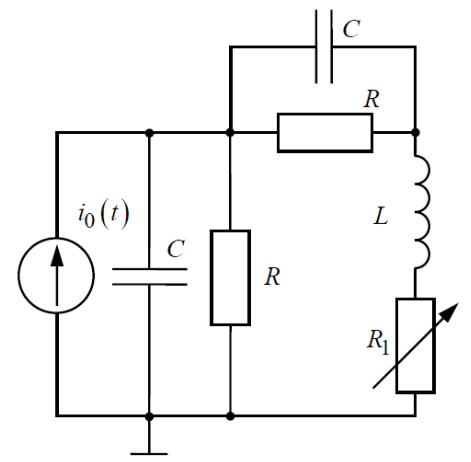
\includegraphics[width=6.5cm]{scheme_third_order.png}
    \caption{Схема для исследования}
    \label{fig:scheme_third_order}
\end{figure}

Соберём схему, изображённую на рис. \ref*{fig:scheme_third_order}.
$C = 0.02\ \text{мкФ}$, $R_1 = 1\ \text{кОм}$, $R_1 = 1\ \text{кОм}$,
$L = 25\ \text{мГн}$.

Полученная осциллограмма напряжения на входе представлена на
рис. \ref*{fig:oscillograph_third_order}.

\begin{figure}[!h]
    \centering
    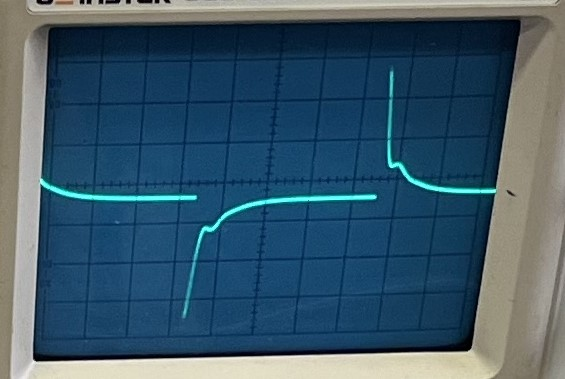
\includegraphics[width=0.6\textwidth]{oscillograph_third_order_IMG_7898.JPG}
    \caption{Осциллограмма напряжения на входе}
    \label{fig:oscillograph_third_order}
\end{figure}

\subsubsection{Теоретические расчеты}

Исходя из данных цепи найдем собственные частоты

\[
    p_{1} = -\alpha_1 =
    -\frac{1}{R C}
    = -\frac{1}{5\cdot 10^{3} \cdot 0.02 \cdot 10^{-6}}
    = -10\ \text{кГц}
\]

\[
    \alpha_2
    = \frac{1}{2} \left( \frac{R_1}{L} + \frac{1}{R C} \right)
    = \frac{1}{2} \left(
    \frac{1 \cdot 10^{3} }{25 \cdot 10^{-3}}
    + \frac{1}{5 \cdot 10^{3} \cdot 0.02 \cdot 10^{-6}}
    \right)
    = 25\ \text{кГц}
\]

\[
    \begin{aligned}
        p_{2,3} & = -\alpha_2 \pm \sqrt{\alpha_2^2 - \frac{2+R_1/R}{L C}} = \\
                & = -25 \cdot 10^3 \pm \sqrt{
            (25 \cdot 10^3)^2 - \frac{2+1/5}{25 \cdot 10^{-3} \cdot 0.02 \cdot 10^{-6}}
        }
        = -25  \pm 61j\ \text{кГц}
    \end{aligned}
\]


\subsubsection{Вопросы}

7. Каким аналитическим выражением описывается осциллографируемый
процесс?

\[
    u(t) = A_1 e^{p_1 t} + A_2 e^{p_2 t} + A_3 e^{p_3 t},
\]
где собственные частоты $p_{1,2,3}$ могут быть а) тремя действительными,
б) двумя действительными и одним комплексным.

8. Каковы значения вычисленных собственных частот,
и соответствует ли этим значениям снятая осциллограмма?

\[
    p_1 = -10\ \text{кГц},\ p_2 = -25 + 61j\ \text{кГц},\
    p_3 = -25 - 61j\ \text{кГц}
\]

Согласно аналитическуму выражению и полученым значениям собственных
частот, осциллограмма должна представлять собой сумму затухающей экспоненты и колебательного процесса,
что и наблюдается на рис. \ref*{fig:oscillograph_third_order}.
